\documentclass{../../../oss-apphys}

\begin{document}
\genheader

\gentitle{2}{LIGHT AND GEOMETRIC OPTICS}

\genmultidirections

\gengravity

\raggedcolumns
\begin{multicols}{2}

  \begin{enumerate}[leftmargin=18pt]  
  \item Two satellites of equal mass orbit a planet. Satellite B orbits at twice
    the orbital radius of Satellite A. Which of the following statements is
    true?
    \begin{enumerate}[noitemsep,topsep=0pt,leftmargin=18pt,label=(\Alph*)]
    \item The gravitational force on Satellite A is four times less than that on
      Satellite B.
    \item The gravitational force on Satellite A is two times less than that on
      Satellite B.
    \item The gravitational force on the satellites is equal.
    \item The gravitational force on Satellite A is two times greater than that
      on Satellite B.
    \item The gravitational force on Satellite A is four times greater than that
      on Satellite B.
    \end{enumerate}
    
  \item A $70$-\si{\kilo\gram} astronaut floats at a distance of \SI{10}{\metre}
    from a $50000$-\si{\kilo\gram} spacecraft. What is the force of attraction
    between the astronaut and spacecraft?
    \begin{enumerate}[noitemsep,topsep=0pt,leftmargin=18pt,label=(\Alph*)]
    \item\SI{2.4e-6}{\newton}
    \item\SI{2.4e-5}{\newton}
    \item Zero; there is no gravity in space.
    \item\SI{2.4e5}{\newton}
    \item\SI{2.4e6}{\newton}
    \end{enumerate}
    
  \item The centripetal acceleration on \SI{1000}{\kilo\gram} car in a turn is
    \SI{1e5}{m/s^2}. The radius of the turn is \SI{10}{\metre}. What is the
    car's speed?
    \begin{enumerate}[noitemsep,topsep=0pt,leftmargin=18pt,label=(\Alph*)]
    \item\SI{1e1}{\metre\per\second}
    \item\SI{1e2}{\metre\per\second}
    \item\SI{1e3}{\metre\per\second}
    \item\SI{1e4}{\metre\per\second}
    \item\SI{1e5}{\metre\per\second}
    \end{enumerate}

    \columnbreak
    
  \item A proposed ``space elevator'' can lift a \SI{1000}{\kilo\gram} payload
    to an orbit of \SI{150}{\kilo\metre} above the Earth's surface. The radius
    of the Earth is \SI{6.4e6}{\metre}, and the Earth's mass is
    \SI{6.e24}{\kilo\gram}. What is the gravitational potential energy of the
    payload when it reaches orbit?
    \begin{enumerate}[noitemsep,topsep=0pt,leftmargin=18pt,label=(\Alph*)]
    \item\SI{1.0e3}{\joule}
    \item\SI{2.7e6}{\joule}
    \item\SI{6.1e10}{\joule}
    \item\SI{2.7e12}{\joule}
    \item\SI{1.0e15}{\joule}
    \end{enumerate}

  \item The Earth is at an average distance of \SI{1}{AU} from the Sun and has
    an orbital period of \SI{1}{year}. Jupiter orbits the Sun at approximately
    \SI{5}{AU}. About how long is the orbital period of Jupiter?
    \begin{enumerate}[noitemsep,topsep=0pt,leftmargin=18pt,label=(\Alph*)]
    \item\SI{1}{year}
    \item\SI{2}{years}
    \item\SI{5}{years}
    \item\SI{11}{years}
    \item\SI{125}{years}
    \end{enumerate}

  \item A satellite orbits the Earth at a distance of \SI{200}{\km}. If the mass
    of the Earth is \SI{6.e24}{\kilo\gram} and the Earth's radius is
    \SI{6.4e6}{\metre}, what is the satellite's speed?
    \begin{enumerate}[noitemsep,topsep=0pt,leftmargin=18pt,label=(\Alph*)]
    \item\SI{1.e3}{\metre\per\second}
    \item\SI{3.5e3}{\metre\per\second}
    \item\SI{7.8e3}{\metre\per\second}
    \item\SI{5e6}{\metre\per\second}
    \item\SI{6.1e7}{\metre\per\second}
    \end{enumerate}

    \columnbreak

  \item Mars orbits the Sun at a distance of \SI{2.3e11}{\metre}. The mass of
    the Sun is \SI{2.e30}{\kilo\gram}, and the mass of Mars is
    \SI{6.4e23}{\kilo\gram}. Approximately what is the gravitational force that
    the Sun exerts on Mars?
    \begin{enumerate}[noitemsep,topsep=0pt,leftmargin=18pt,label=(\Alph*)]
    \item\SI{1.6e20}{\newton}
    \item\SI{1.6e21}{\newton}
    \item\SI{3.7e21}{\newton}
    \item\SI{3.7e32}{\newton}
    \item\SI{3.7e42}{\newton}
    \end{enumerate}

  \item When climbing from sea level to the top of Mount Everest, a hiker
    changes elevation by \SI{8848}{\metre}. By what percentage will the
    gravitational field of the Earth change during the climb? (The Earth's
    mass is \SI{6.e24}{\kilo\gram}, and its radius is \SI{6.4e6}{\metre}.)
    \begin{enumerate}[noitemsep,topsep=0pt,leftmargin=18pt,label=(\Alph*)]
    \item It will increase by approximately \SI{0.3}{\percent}.
    \item It will decrease by approximately \SI{0.3}{\percent}.
    \item It will increase by approximately \SI{12}{\percent}.
    \item It will decrease by approximately \SI{12}{\percent}.
    \item The gravitational field strength will not change.
    \end{enumerate}

  \item Four planets, A through D, orbit the same star. The relative masses and
    distances from the star for each planet are shown in the table. For
    example, Planet A has twice the mass of Planet B, and Planet D has
    three times the orbital radius of Planet A. Which planet has the highest
    gravitational attraction to the star?
    \begin{center}
      \vspace{-.1in}
      \begin{tabular}{lll}
        \hline
        \textbf{Planet} & \textbf{Relative mass} & \textbf{Relative distance}\\
        \hline
        A\hspace{.4in}& $2m$     & $r$    \\ \hline
        B & $m$                  & $0.1r$\hspace{.25in} \\ \hline
        C & $0.5m$\hspace{.25in} & $2r$   \\ \hline
        D & $4m$                 & $3r$   \\ \hline
      \end{tabular}
    \end{center}
    \begin{enumerate}[noitemsep,topsep=0pt,leftmargin=18pt,label=(\Alph*)]
    \item Planet A
    \item Planet B
    \item Planet C
    \item Planet D
    \item All have the same gravitational attraction to the star.
    \end{enumerate}

    \columnbreak
    
  \item A satellite orbits the Earth at a distance that is four times the radius
    of the Earth. If the acceleration due to gravity near the surface of the
    Earth is $g$, the acceleration of the satellite is most nearly
    \begin{enumerate}[noitemsep,topsep=0pt,leftmargin=18pt,label=(\Alph*)]
    \item zero
    \item $g/2$
    \item $g/4$
    \item $g/8$
    \item $g/16$
    \end{enumerate}

  \item The mass of a planet is $1/4$ that of Earth and its radius is half of
    Earth's radius. The acceleration due to gravity on this planet is most
    nearly
    \begin{enumerate}[noitemsep,topsep=0pt,leftmargin=18pt,label=(\Alph*)]
    \item\SI{2 }{\metre\per\second^2}
    \item\SI{4 }{\metre\per\second^2}
    \item\SI{5 }{\metre\per\second^2}
    \item\SI{10}{\metre\per\second^2}
    \item\SI{20}{\metre\per\second^2}
    \end{enumerate}
  
  \item A satellite orbits the Earth in an elliptical orbit, with point A being
    close to the Earth and point B farther away. As the satellite moves from
    point A to point B, which of the following is true of the angular momentum
    and kinetic energy of the satellite?
    \begin{center}
      \vspace{-.1in}
      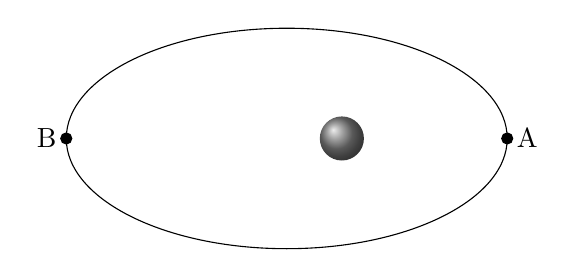
\begin{tikzpicture}[scale=1.4]
        \tikzstyle{balloon}=[ball color=gray];
        \draw(0,0) ellipse (2 and 1);
        \draw[fill=black](2,0) circle(0.05) node[right]{A};
        \draw[fill=black](-2,0) circle(0.05) node[left]{B};
        \shade[balloon] (0.5,0) circle (0.2);
      \end{tikzpicture}
    \end{center}
  
    \begin{tabular}{lll}
      & \underline{Angular momentum} & \underline{Kinetic energy}\\
      (a) & Increases & Remains constant \\
      (b) & Remains constant & Increases \\
      (c) & Decreases & Remains constant \\
      (d) & Remains constant & Decreases \\
      (e) & Remains constant & Remains constant
    \end{tabular}

    \columnbreak
    
  \item Two planets of mass $M$ and $9M$ are in the same solar system. The
    radius of the planet of mass $M$ is $R$. In order for the acceleration due
    to gravity to be the same for each planet, the radius of the planet of mass
    $9M$ would have to be
    \begin{enumerate}[noitemsep,topsep=0pt,leftmargin=18pt,label=(\Alph*)]
    \item $R/2$
    \item $R$
    \item $2R$
    \item $3R$
    \item $9R$
    \end{enumerate}
    %\vspace{-.5in}
    
  \item Two planets, X and Y, orbit a star. Planet X orbits at a radius $R$, and
    Planet Y orbits at a radius $3R$. Which of the following best represents
    the relationship between the acceleration $a_X$ of Planet X and the
    acceleration $a_Y$ of Planet Y?
    \begin{center}
      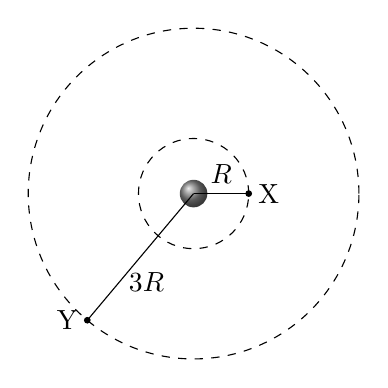
\begin{tikzpicture}[scale=.7]
        \tikzstyle{balloon}=[ball color=gray];
        \shade[balloon](0,0) circle(.25);
        \draw[dashed](0,0) circle(1);
        \draw[dashed](0,0) circle(3);
        \draw(0,0)--(1,0) node[pos=1,right]{X} node[midway,above]{$R$};
        \draw[fill=black](1,0) circle(.05);
        \begin{scope}[rotate=230]
          \draw(0,0)--(3,0) node[pos=1,left]{Y} node[pos=0.7,right]{$3R$};
          \draw[fill=black](3,0) circle(.05);
        \end{scope}
      \end{tikzpicture}
    \end{center}
    \begin{enumerate}[noitemsep,topsep=0pt,leftmargin=18pt,label=(\Alph*)]
    \item $a_X = 9a_Y$
    \item $9a_X = a_Y$
    \item $a_X = 3a_Y$
    \item $3a_X = a_Y$
    \item $a_X = a_Y$
    \end{enumerate}
  \item A satellite is in a stable circular orbit around the Earth at a radius
    $R$ and speed $v$. At what radius would the satellite travel in a stable
    orbit with a speed $2v$?
    \begin{enumerate}[noitemsep,topsep=0pt,leftmargin=18pt,label=(\Alph*)]
    \item $1⁄4\;R$
    \item $1⁄2\;R$
    \item $R$
    \item $2R$
    \item $4R$
    \end{enumerate}

    \columnbreak

  \item The Earth and the moon apply a gravitational force to each other.
    Which of the following statements is true?
    \begin{enumerate}[noitemsep,topsep=0pt,leftmargin=18pt,label=(\Alph*)]
    \item The Earth applies a greater force on the moon than the moon exerts on
      the Earth.
    \item The Earth applies a smaller force on the moon than the moon exerts on
      the Earth.
    \item The Earth applies a force on the moon, but the moon does not exert a
      force on the Earth.
    \item The Earth does not apply a force on the moon, but the moon exerts a
      force on the Earth.
    \item The force the Earth applies to the moon is equal and opposite to the
      force the moon applies to the Earth.
    \end{enumerate}

  \item Two masses exert a gravitational force $F$ on each other. If one of the
    masses is doubled, and the distance between the masses is tripled, the
    new force between them is
    \begin{enumerate}[noitemsep,topsep=0pt,leftmargin=18pt,label=(\Alph*)]
    \item $6F$
    \item $2F/3$
    \item $2F/9$
    \item $3F/2$
    \item $4F/9$
    \end{enumerate}

  \item A planet orbits at a radius $R$ around a star of mass $M$. The period of
    orbit of the planet is
    \begin{enumerate}[noitemsep,topsep=0pt,leftmargin=18pt,label=(\Alph*)]
    \item $\displaystyle\sqrt{\frac{4\pi^2R^2}{GM}}$
    \item $\displaystyle\frac{4\pi^2R^3}{GM}$
    \item $\displaystyle\sqrt{\frac{4\pi^2R^3}{GM}}$
    \item $\displaystyle\sqrt{\frac{4\pi^2R}{GM}}$
    \item $\displaystyle\frac{GM}{4\pi^2R}$
    \end{enumerate}

    \columnbreak

  \item A moon orbits a large planet in an elliptical orbit, with its closest
    approach at a distance $a$, and its farthest distance $b$. The speed of the
    moon at point b is $v$. The speed at point $a$ is
    \begin{enumerate}[noitemsep,topsep=0pt,leftmargin=18pt,label=(\Alph*)]
    \item $\displaystyle\frac{av}{b}$
    \item $\displaystyle\frac{bv}{a}$
    \item $\displaystyle\frac{(a+b)v}{b}$
    \item $\displaystyle\frac{(b-a)v}{b}$
    \item $\displaystyle\frac{2bv}{a}$
    \end{enumerate}

  \item A satellite orbits the Earth in an elliptical orbit. Which of the
    following statements is true?
    \begin{enumerate}[noitemsep,topsep=0pt,leftmargin=18pt,label=(\Alph*)]
    \item The angular velocity of the satellite increases as it travels farther
      from the Earth.
    \item The acceleration of the satellite increases as it travels closer to
      the Earth.
    \item The angular momentum of the satellite increases as it travels closer
      to the Earth.
    \item The potential energy of the satellite is equal to its kinetic energy
      at all points in the orbit.
    \item The speed of the satellite must remain constant for it to remain
      in orbit around the Earth.
    \end{enumerate}

  \item Two moons of mass $m$ and $2m$ orbit a planet of mass $M$
    at the same radius $R$ and speed $v$ toward each other, as shown. The moons
    collide and stick together without destroying either moon. The total
    momentum of the moons after the collision is
    \begin{center}
      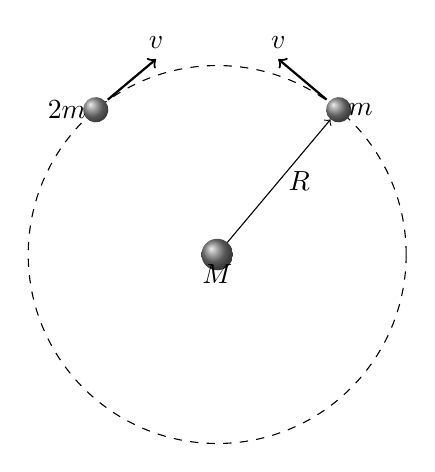
\begin{tikzpicture}[scale=0.8]
        \tikzstyle{balloon}=[ball color=gray];
        \shade[balloon] circle(.25) node[below]{$M$};
        \draw[dashed](0,0) circle(3);
        \begin{scope}[rotate=50]
          \draw[->](0.25,0)--(2.8,0) node[midway,right]{$R$};
          \shade[balloon] (3,0) circle (0.2) node[right]{$m$};
          \draw[thick,->](3,0.25)--(3,1.25) node[pos=1,above]{$v$};
        \end{scope}
        \begin{scope}[rotate=130]
          \shade[balloon] (3,0) circle (0.2) node[left]{$2m$};
          \draw[thick,->](3,-0.25)--(3,-1.25) node[pos=1,above]{$v$};
        \end{scope}
      \end{tikzpicture}
    \end{center}
    \begin{enumerate}[noitemsep,topsep=0pt,leftmargin=18pt,label=(\Alph*)]
    \item $mv$
    \item $2mv$
    \item $3mv$
    \item $6mv$
    \item zero
    \end{enumerate}

    \columnbreak
    
  \item The velocity of the two masses after the collision above is
    \begin{enumerate}[noitemsep,topsep=0pt,leftmargin=18pt,label=(\Alph*)]
    \item $v$ counterclockwise
    \item $v/2$ counterclockwise
    \item $v/2$ clockwise
    \item $v/3$ counterclockwise
    \item $v/3$ clockwise
    \end{enumerate}

  \item Consider a two-star system shown above, which consists of two stars of
    mass $m$ rotating in a circle of radius $r$ about their center of mass. What
    is the total energy of the two-star system?
    \begin{enumerate}[noitemsep,topsep=0pt,leftmargin=18pt,label=(\Alph*)]
    \item $-Gm^2/2r$
    \item $Gm^2/2r$
    \item $Gm^2/4r$
    \item $3Gm^2/4r$
    \item $-Gm^2/4r$
    \end{enumerate}

  \item If a planet has twice the radius of Earth and half of Earth's density,
    what is the acceleration due to gravity on the surface of the planet (in
    terms of the gravitational acceleration $g$ on the surface of Earth)?
    \begin{enumerate}[noitemsep,topsep=0pt,leftmargin=18pt,label=(\Alph*)]
    \item $4g$
    \item $2g$
    \item $g$
    \item $g/2$
    \item $g/4$
    \end{enumerate}
  \end{enumerate}
\end{multicols}

\newpage
%\genanswersheet{1 \& C}{Simple Harmonic Motion and Universal Gravitation}
%
%\begin{center}
%  \begin{minipage}[t]{.2\textwidth}
%    \vspace{.2in}
%    \bgroup
%    \begin{tabular}{>{\centering}m{1.3cm} >{\centering}m{1.7cm}}
%      No. & Answer
%    \end{tabular}\\
%    \def\arraystretch{1.5}
%    \begin{tabular}{|>{\centering}m{1.3cm}|>{\centering}m{1.7cm}|}
%      \hline
%      1 & \\ \hline
%      2 & \\ \hline
%      3 & \\ \hline
%      4 & \\ \hline
%      5 & \\ \hline
%      6 & \\ \hline
%      7 & \\ \hline
%      8 & \\ \hline
%      9 & \\ \hline
%      10 & \\ \hline
%      11 & \\ \hline
%      12 & \\ \hline
%      13 & \\ \hline
%      14 & \\ \hline
%      15 & \\ \hline
%      16 & \\ \hline
%      17 & \\ \hline
%      18 & \\ \hline
%      19 & \\ \hline
%      20 & \\ \hline
%      21 & \\ \hline
%      22 & \\ \hline
%      23 & \\ \hline
%      24 & \\ \hline
%      25 & \\ \hline
%    \end{tabular}
%    \egroup
%  \end{minipage}
%  \hspace{.5in}
%  \begin{minipage}[t]{.2\textwidth}
%    \vspace{.2in}
%    \bgroup
%    \begin{tabular}{>{\centering}m{1.3cm} >{\centering}m{1.7cm}}
%      No. & Answer
%    \end{tabular}\\
%    \def\arraystretch{1.5}
%    \begin{tabular}{|>{\centering}m{1.3cm}|>{\centering}m{1.7cm}|}
%      \hline
%      26 & \\ \hline
%      27 & \\ \hline
%      28 & \\ \hline
%      29 & \\ \hline
%      30 & \\ \hline
%      31 & \\ \hline
%      32 & \\ \hline
%      33 & \\ \hline
%      34 & \\ \hline
%      35 & \\ \hline
%      36 & \\ \hline
%      37 & \\ \hline
%      38 & \\ \hline
%    \end{tabular}
%    \egroup
%  \end{minipage}
%\end{center}
%\newpage

\genfreetitle{2}{LIGHT AND GEOMETRIC OPTICS}{5}

\genfreedirections{10}

% THIS IS TAKEN FROM THE 2001 AP PHYSICS B EXAM FREE-RESPONSE QUESTION #4
\begin{center}
  \pic{.4}{glass1.png}
\end{center}
\begin{enumerate}[leftmargin=15pt]
\item In an experiment a beam of red light of wavelength 675 nm in air passes
  from glass into air, as shown above. The incident and refracted angles are
  $\theta_1$ and $\theta_2$, respectively. In the experiment, angle $\theta_2$
  is measured for various angles of incidence $\theta_1$, and the sines of the
  angles are used to obtain the line shown in the following graph.
  \begin{center}
    \pic{.6}{graph1.png}
  \end{center}
  \begin{enumerate}[noitemsep]
  \item Assuming an index of refraction of 1.00 for air, use the graph to
    determine a value for the index of refraction of the glass for the red
    light. Explain how you obtained this value.
    \newpage
    
  \item For this red light, determine the following.
    \begin{enumerate}[noitemsep]
    \item The frequency in air
    \item The speed in glass
    \item The wavelength in glass
    \end{enumerate}
    
  \item The index of refraction of this glass is 1.66 for violet light, which
    has wavelength 425 nm in air.
    \begin{enumerate}[noitemsep]
    \item Given the same incident angle $\theta_1$ , show on the ray diagram on
      the previous page how the refracted ray for the violet light would vary
      from the refracted ray already drawn for the red light.
    \item Sketch the graph of $\sin\theta_2$ versus $\sin\theta_1$ for the
      violet light on the figure on the previous page that shows the same graph
      already drawn for the red light.
    \end{enumerate}

  \item Determine the critical angle of incidence $\theta_c$for the violet
    light in the glass in order for total internal reflection to occur.
  \end{enumerate}
  \vspace{1.5in}
  
  % THIS IS TAKEN FROM THE 2005 AP PHYSICS B EXAM FREE-RESPONSE QUESTION #4
\item Your teacher gives you a slide with two closely spaced slits on it. She
  also gives you a laser with a wavelength $\lambda=\SI{632}{\nano\metre}$. The
  laboratory task that you are assigned asks you to determine the spacing
  between the slits. These slits are so close together that you cannot measure
  their spacing with a typical measuring device.
  \begin{enumerate}[noitemsep]
  \item From the list below, select the additional equipment you will need to
    do your experiment by checking the line next to each item.
    \begin{multicols}{3}
      \underline{\hspace{.3in}} Meterstick\\
      \underline{\hspace{.3in}} Ruler\\
      \underline{\hspace{.3in}} Tape measure\\
      \underline{\hspace{.3in}} Light-intensity meter\\
      \columnbreak
      
      \underline{\hspace{.3in}} Large screen\\
      \underline{\hspace{.3in}} Paper\\
      \underline{\hspace{.3in}} Slide holder\\
      \underline{\hspace{.3in}} Stopwatch
    \end{multicols}
  \item Draw a labeled diagram of the experimental setup that you would use. On
    the diagram, use symbols to identify carefully what measurements you will
    need to make.
    \begin{center}
      \begin{tikzpicture}[scale=.45]
        \draw[thick,->](-10,0)--(10,0) node[pos=1,right]{Position};
        \draw[thick,->](0,-7)--(0,7) node[pos=1,right]{Position};
      \end{tikzpicture}
    \end{center}
  \item On the axes below, sketch a graph of intensity versus position that
    would be produced by your setup, assuming that the slits are very narrow
    compared to their separation.
  \end{enumerate}
  \vspace{2in}
  
  % THIS IS TAKEN FROM THE 2014 AP PHYSICS B EXAM FREE-RESPONSE QUESTION #7
  \begin{center}
    \pic{.35}{film1.png}\\
    \underline{Note:} Figure not drawn to scale.
  \end{center}
\item A thin layer of transparent oil is placed on top of a transparent plate.
  The oil film is then illuminated by white light shining onto the oil's
  surface, as shown in the figure above. To an observer standing right next to
  the light source and looking straight down on the oil film, the oil film
  appears green, corresponding to a wavelength of 520 nm in air. The oil has an
  index of refraction of 1.52.
  \begin{enumerate}[noitemsep]
  \item Determine the frequency of the green light in the air.
    \vspace{.25in}
  \item Determine the frequency of the green light in the oil film.
    \vspace{.25in}
  \item Calculate the wavelength of the green light in the oil film.
    \vspace{.25in}
  \item The oil film thickness is half of the wavelength you found in part (c).
    Is the index of refraction of the plate greater than, less than, or equal
    to that of the oil?

    \vspace{.1in}
    \underline{\hspace{.3in}} Greater than\hspace{.2in}
    \underline{\hspace{.3in}} Less than\hspace{.2in}
    \underline{\hspace{.3in}} Equal to
    
    \vspace{.1in}Justify your answer.

    \begin{center}
      \pic{.7}{film2.png}\\
      \underline{Note:} Figure not drawn to scale.
    \end{center}
  \item As the observer starts moving to the right away from the light source,
    as shown in the figures above, the film appears to change color. Describe
    the color change and give an explanation for this phenomenon.
  \end{enumerate}
\end{enumerate}
\end{document}
